%----------
%   IMPORTANTE
%----------

% Si nunca has utilizado LaTeX es conveniente que aprendas una serie de conceptos básicos antes de utilizar esta plantilla. Te aconsejamos que leas previamente algún tutorial (puedes encontar muchos en Internet).

% Esta plantilla está basada en las recomendaciones de la guía "Trabajo fin de Máster: Escribir el TFM", que encontrarás en http://uc3m.libguides.com/TFM/escribir
% contiene recomendaciones de la Biblioteca basadas principalmente en estilos APA e IEEE, pero debes seguir siempre las orientaciones de tu Tutor de TFM y la normativa de TFM para tu titulación.

% Encontrarás un ejemplo de TFM realizado con esta misma plantilla en la carpeta "_ejemplo_TFM_2019". Consúltalo porque contiene ejemplos útiles para incorporar tablas, figuras, listados de código, bibliografía, etc.


%----------
%	CONFIGURACIÓN DEL DOCUMENTO
%----------

% Definimos las características del documento y añadimos una serie de paquetes (\usepackage{package}) que agregan funcionalidades a LaTeX.

\documentclass[12pt]{report} %fuente a 12pt

% MÁRGENES: 2,5 cm sup. e inf.; 3 cm izdo. y dcho.
\usepackage[
a4paper,
vmargin=2.5cm,
hmargin=2.7cm
]{geometry}

% INTERLINEADO: Estrecho (6 ptos./interlineado 1,15) o Moderado (6 ptos./interlineado 1,5)
\renewcommand{\baselinestretch}{1.15}
\parskip=6pt

% DEFINICIÓN DE COLORES para portada y listados de código
\usepackage[table]{xcolor}
\definecolor{azulUC3M}{RGB}{0,0,102}
\definecolor{gray97}{gray}{.97}
\definecolor{gray75}{gray}{.75}
\definecolor{gray45}{gray}{.45}

% Soporte para GENERAR PDF/A --es importante de cara a su inclusión en e-Archivo porque es el formato óptimo de preservación y a la generación de metadatos, tal y como se describe en http://uc3m.libguides.com/ld.php?content_id=31389625. En la carpeta incluímos el archivo plantilla_tfg_2017.xmpdata en el que puedes incluir los metadatos que se incorporarán al archivo PDF cuando lo compiles. Ese archivo debe llamarse igual que tu archivo .tex. Puedes ver un ejemplo en esta misma carpeta.
\usepackage[a-1b]{pdfx}

% ENLACES
\usepackage{hyperref}
\hypersetup{colorlinks=true,
	linkcolor=black, % enlaces a partes del documento (p.e. índice) en color negro
	urlcolor=blue} % enlaces a recursos fuera del documento en azul

% EXPRESIONES MATEMATICAS
\usepackage{amsmath,amssymb,amsfonts,amsthm}

\usepackage{txfonts} 
\usepackage[T1]{fontenc}
\usepackage[utf8]{inputenc}

\usepackage[english]{babel} 
\usepackage[babel, english=american]{csquotes}
\AtBeginEnvironment{quote}{\small}

% diseño de PIE DE PÁGINA
\usepackage{fancyhdr}
\pagestyle{fancy}
\fancyhf{}
\renewcommand{\headrulewidth}{0pt}
\rfoot{\thepage}
\fancypagestyle{plain}{\pagestyle{fancy}}

% DISEÑO DE LOS TÍTULOS de las partes del trabajo (capítulos y epígrafes o subcapítulos)
\usepackage{titlesec}
\usepackage{titletoc}
\titleformat{\chapter}[block]
{\large\bfseries\filcenter}
{\thechapter.}
{5pt}
{\MakeUppercase}
{}
\titlespacing{\chapter}{0pt}{0pt}{*3}
\titlecontents{chapter}
[0pt]                                               
{}
{\contentsmargin{0pt}\thecontentslabel.\enspace\uppercase}
{\contentsmargin{0pt}\uppercase}                        
{\titlerule*[.7pc]{.}\contentspage}                 

\titleformat{\section}
{\bfseries}
{\thesection.}
{5pt}
{}
\titlecontents{section}
[5pt]                                               
{}
{\contentsmargin{0pt}\thecontentslabel.\enspace}
{\contentsmargin{0pt}}
{\titlerule*[.7pc]{.}\contentspage}

\titleformat{\subsection}
{\normalsize\bfseries}
{\thesubsection.}
{5pt}
{}
\titlecontents{subsection}
[10pt]                                               
{}
{\contentsmargin{0pt}                          
	\thecontentslabel.\enspace}
{\contentsmargin{0pt}}                        
{\titlerule*[.7pc]{.}\contentspage}  


% DISEÑO DE TABLAS. Puedes elegir entre el estilo para ingeniería o para ciencias sociales y humanidades. Por defecto, está activado el estilo de ingeniería. Si deseas utilizar el otro, comenta las líneas del diseño de ingeniería y descomenta las del diseño de ciencias sociales y humanidades
\usepackage{multirow} %permite combinar celdas 
\usepackage{caption} %para personalizar el título de tablas y figuras
\usepackage{floatrow} %utilizamos este paquete y sus macros \ttabbox y \ffigbox para alinear los nombres de tablas y figuras de acuerdo con el estilo definido. Para su uso ver archivo de ejemplo 
\usepackage{array} % con este paquete podemos definir en la siguiente línea un nuevo tipo de columna para tablas: ancho personalizado y contenido centrado
\newcolumntype{P}[1]{>{\centering\arraybackslash}p{#1}}
\DeclareCaptionFormat{upper}{#1#2\uppercase{#3}\par}

% Diseño de tabla para ingeniería
\captionsetup[table]{
	format=upper,
	justification=centering,
	labelsep=period,
	width=.75\linewidth,
	labelfont=small,
	font=small,
}

%Diseño de tabla para ciencias sociales y humanidades
%\captionsetup[table]{
%	justification=raggedright,
%	labelsep=period,
%	labelfont=small,
%	singlelinecheck=false,
%	font={small,bf}
%}


% DISEÑO DE FIGURAS. Puedes elegir entre el estilo para ingeniería o para ciencias sociales y humanidades. Por defecto, está activado el estilo de ingeniería. Si deseas utilizar el otro, comenta las líneas del diseño de ingeniería y descomenta las del diseño de ciencias sociales y humanidades
\usepackage{graphicx}
\graphicspath{{images/}} %ruta a la carpeta de imágenes

% Diseño de figuras para ingeniería
\captionsetup[figure]{
	format=hang,
	name=Fig.,
	justification=centering,
	singlelinecheck=off,
	labelsep=colon,
	labelfont=small,
	font=small		
}

% Diseño de figuras para ciencias sociales y humanidades
%\captionsetup[figure]{
%	format=hang,
%	name=Figure,
%	singlelinecheck=off,
%	labelsep=period,
%	labelfont=small,
%	font=small		
%}


% NOTAS A PIE DE PÁGINA
\usepackage{chngcntr} %para numeración contínua de las notas al pie
\counterwithout{footnote}{chapter}

% LISTADOS DE CÓDIGO
% soporte y estilo para listados de código. Más información en https://es.wikibooks.org/wiki/Manual_de_LaTeX/Listados_de_código/Listados_con_listings
\usepackage{listings}

% definimos un estilo de listings
\lstdefinestyle{estilo}{ frame=Ltb,
	framerule=0pt,
	aboveskip=0.5cm,
	framextopmargin=3pt,
	framexbottommargin=3pt,
	framexleftmargin=0.4cm,
	framesep=0pt,
	rulesep=.4pt,
	backgroundcolor=\color{gray97},
	rulesepcolor=\color{black},
	%
	basicstyle=\ttfamily\footnotesize,
	keywordstyle=\bfseries,
	stringstyle=\ttfamily,
	showstringspaces = false,
	commentstyle=\color{gray45},     
	%
	numbers=left,
	numbersep=15pt,
	numberstyle=\tiny,
	numberfirstline = false,
	breaklines=true,
	xleftmargin=\parindent
}

\captionsetup[lstlisting]{font=small, labelsep=period}
% fijamos el estilo a utilizar 
\lstset{style=estilo}
\renewcommand{\lstlistingname}{\uppercase{Código}}


%BIBLIOGRAFÍA - PUEDES ELEGIR ENTRE ESTILO IEEE O APA. POR DEFECTO ESTÁ CONFIGURADO IEEE. SI DESEAS USAR APA, COMENTA LAS LÍNEA DE IEEE Y DESCOMENTA LAS DE APA. Si haces cambios en la configuración de la bibliografía y no obtienes los resultados esperados, es recomendable limpiar los archivos auxiliares y volver a compilar en este orden: COMPILAR-BIBLIOGRAFIA-COMPILAR
% Tienes más información sobre cómo generar bibliografía en http://tex.stackexchange.com/questions/154751/biblatex-with-biber-configuring-my-editor-to-avoid-undefined-citations , https://es.sharelatex.com/learn/Bibliography_management_in_LaTeX y en http://www.ctan.org/tex-archive/macros/latex/exptl/biblatex-contrib
% También te recomendamos consultar la guía temática de la Biblioteca sobre citas bibliográficas: http://uc3m.libguides.com/guias_tematicas/citas_bibliograficas/inicio

% CONFIGURACIÓN PARA LA BIBLIOGRAFÍA IEEE
\usepackage[backend=biber, style=ieee, isbn=false,sortcites, maxbibnames=5, minbibnames=1]{biblatex} % Configuración para el estilo de citas de IEEE, recomendado para el área de ingeniería. "maxbibnames" indica que a partir de 5 autores trunque la lista el primero (minbibnames) y añada "et al." tal y como se utiliza en el estilo IEEE.

%CONFIGURACIÓN PARA LA BIBLIOGRAFÍA APA
%\usepackage[style=apa, backend=biber, natbib=true, hyperref=true, uniquelist=false, sortcites]{biblatex}
%\DeclareLanguageMapping{spanish}{spanish-apa}

\addbibresource{citations/websites.bib} % llama al archivo bibliografia.bib que utilizamos de ejemplo


%-------------
%	DOCUMENTO
%-------------

\begin{document}
\pagenumbering{roman} % Se utilizan cifras romanas en la numeración de las páginas previas al cuerpo del trabajo
	
%----------
%	PORTADA
%----------	
\begin{titlepage}
	\begin{sffamily}
	\color{azulUC3M}
	\begin{center}
		\begin{figure}[H] %incluimos el logotipo de la Universidad
			\makebox[\textwidth][c]{
\includegraphics[width=16cm]{Portada_Logo.png}}
		\end{figure}
		\vspace{1cm}
		\begin{Large}
			Master in Big Data Analytics\\			
			Academic Year 2022-2023\\
			\vspace{1cm}		
			\textsl{Master Thesis}
			\bigskip
			
		\end{Large}
		 	{\Huge ``Thesis title''}\\
		 	\vspace*{0.5cm}
	 		\rule{10.5cm}{0.1mm}\\
			\vspace*{0.9cm}
			{\LARGE Author's complete name}\\ 
			\vspace*{1cm}
		\begin{Large}
			1st Tutor complete name\\
			2nd Tutor complete name\\
			Place and date\\
		\end{Large}
	\end{center}
	
	\vfill
	\color{black}
	\begin{footnotesize}
	\noindent\fbox{
	\begin{minipage}{\textwidth}
		\textbf{AVOID PLAGIARISM}\\
		The University uses the \textbf{Turnitin Feedback Studio} program within the Aula Global for the delivery of student work. This program compares the originality of the work delivered by each student with millions of electronic resources and detects those parts of the text that are copied and pasted. Plagiarizing in a TFM is considered a \textbf{Serious Misconduct}, and may result in permanent expulsion from the University.
	\end{minipage}	
	}
	\vspace*{.5cm}\\	
	\noindent
\includegraphics[width=4.2cm]{images/creativecommons.png}\\
	\emph{[Include this code in case you want your Master Thesis published in Open Access University Repository]}\\
	This work is licensed under Creative Commons \textbf{Attribution – Non Commercial – Non Derivatives}

	\end{footnotesize}
	\end{sffamily}
\end{titlepage}

\newpage %página en blanco o de cortesía
\thispagestyle{empty}
\mbox{}

%----------
%	RESUMEN Y PALABRAS CLAVE
%----------	
\renewcommand\abstractname{\large\uppercase{Summary}}
\begin{abstract}
\thispagestyle{plain}
\setcounter{page}{3}
	
	% ESCRIBIR EL RESUMEN AQUÍ
	
	\textbf{Keywords:}
	% Escribir las palabras clave aquí
	
	\vfill
\end{abstract}
	\newpage %página en blanco o de cortesía
	\thispagestyle{empty}
	\mbox{}


%----------
%	DEDICATORIA
%----------	
\chapter*{Dedication}

\setcounter{page}{5}
	
	% ESCRIBIR LA DEDICATORIA AQUÍ	
		
	\vfill
	
	\newpage %página en blanco o de cortesía
	\thispagestyle{empty}
	\mbox{}
	

%----------
%	ÍNDICES
%----------	

%--
%Índice general
%-
\tableofcontents
\thispagestyle{fancy}

\newpage %página en blanco o de cortesía
\thispagestyle{empty}
\mbox{}

%--
%Índice de figuras. Si no se incluyen, comenta las líneas siguientes
%-
\listoffigures
\thispagestyle{fancy}

\newpage %página en blanco o de cortesía
\thispagestyle{empty}
\mbox{}

%--
%Índice de tablas. Si no se incluyen, comenta las líneas siguientes
%-
\listoftables
\thispagestyle{fancy}

\newpage %página en blanco o de cortesía
\thispagestyle{empty}
\mbox{}



% \input{chapters/02_Planificacion.tex}

% \input{chapters/03_Estado_del_arte.tex}

% \input{chapters/04_Diseno_e_implementacion.tex}

% \input{chapters/05_Experimentacion.tex}

% \input{chapters/06_Conclusiones.tex}


%----------
%	TRABAJO
%----------	
\clearpage
\pagenumbering{arabic} % numeración con múmeros arábigos para el resto de la publicación	

\chapter{Introduction}
%Electricity price forecasting attempts to deduce in advance what the price of electricity will be.
%This is a difficult task, as many factors interfere with it: raw materials (as natural gas, coal or uranium) prices, weather conditions or energy demand.
%Apart, the local and global economic situation or tax policies and regulations approved by the government affect, among others.
%
%In this Master's Thesis we want to perform forecasts of the energy price in the short, medium and long term, studying which variables affect the price in the Spanish market.
%Concretely, we want to study hourly, daily, monthly and yearly aggregations.
%Today, after the covid crisis of previous years and the war in Ukraine, prices have been greatly altered, reaching values that have never been seen before.
%In this situation, the completion of this Thesis makes a lot of sense, as we may discover how the market has changed after these two events.
%
%To achieve this goal the author will first select the variables needed to perform the study, download historical data related with them and apply time series analytics tools, both statistical and machine learning based, to understand the data and make forecasts.
In the current situation of transition to clean energy technologies while immersed in the Ukraine war consequences, electricity price forecasting has become a relevant topic. Energy price affects the entire society, from domestic consumers to big industrial clients; and all the sectors like transport, agriculture or services. But for the agents involved in this market, predicting the future price is as important as knowing which variables are affecting it and how: raw materials (as natural gas, coal or uranium) prices or energy demand are some of them. Apart, the local and global economic situation or tax policies and regulations approved by the governments could affect, among others.

That's why in this Master Thesis the author will perform forecasts and study the variables affecting prices. The analysis will be done in an hourly, daily, monthly and yearly fashion, as the series have different properties on different aggregations. Also, the predictors influence will vary on each. Apart, for the hourly and daily cases, the differences between pre-covid and post-war markets will be analyzed.


\section{Project motivation}
The main motivation is to create a product that can can be used by the different market agents to forecast the future electricity prices and to understand what is affecting them and how.

Apart, for the project author will be useful to understand the particularities of working with time series data and to analyze the state of the art in this field.

\section{Objectives}
The project has the following goals:
\begin{itemize}
    \item \textbf{[OBJ1]} Forecast electricity price in the short, medium and long term.
    \item \textbf{[OBJ2]} Understand which variables affect the electricity price in the short, medium and long term.
\end{itemize}
\chapter{Project planning}
Project planning is very necessary on the IT and Data Science world. Decades ago many projects failed due to the lack of organization, so it's important to use some framework to divide the project in different task and set deadlines.

An appropriate planning ensures that goals are met in due time, assigning the adequate resources and minimizing risks. As Data Science operates in the intersection between Computer Science, Maths and subject expertise, we will apply a Software Engineering development methodology.
They can be classified in two big groups \cite{traditional-vs-agile}:
\begin{itemize}
    \item Traditional: Based on pre-organized phases in which the flow of development is unidirectional. They are adequate for projects with very clear requisites, like the ones in construction, where the client exactly knows what he wants so there won't be major changes in the future.
    \item Agile: They can share the same phases as the traditional ones, but they are applied in an incremental and cyclic fashion. At the end of each cycle, a prototype is delivered to the client so he can review it and propose changes: these kind of methodologies are great for fast-paced industries where requirements change and the final product specifications are not completely clear. This is the case of current software development market.
\end{itemize}
By the nature of this project the author has decided to apply an agile methodology, handing in different deliverables to the project supervisor during its development. Concretely, he will use the SCRUM methodology.

\section{SCRUM methodology}
On this type of agile methodology, three phases are found, as can be seen in Figure \ref{fig:scrum-phases} \cite{schwaber1997scrum}.
\begin{enumerate}
    \item Planning phase: Well-defined process where inputs and outputs are clear. On it, the project is defined indicating some initial requisites.
    \item Sprints: Each one of the cycles we talked about in the beginning of this chapter. On it, the project is developed and integrated with previous sprints. Nevertheless, they are non-linear and flexible and there could be differences in their structure between them. Sprints normally take between 2 and 5 weeks and at their end a deliverable can be handed in to the client: when he is satisfied with the result, the final product has been reached.
    \item Closure: Again, a well-defined process in which the final product is prepared to be delivered to the client.
\end{enumerate}
An important person in SCRUM management is the SCRUM Master, who interacts frequently with the development team and the product owner to ensure that the project fulfills the client needs.

\begin{figure}[H]
\centering
    \caption{SCRUM development methodology phases \cite{schwaber1997scrum}.}
    \label{fig:scrum-phases}
    \fbox{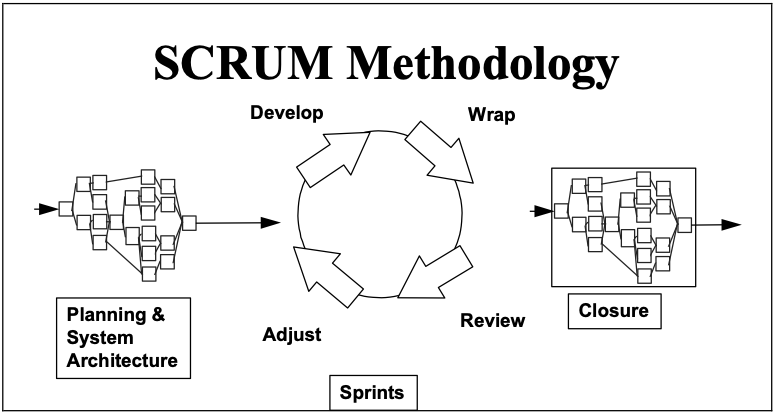
\includegraphics[scale=0.4]{images/planning/scrum_phases}}
\end{figure}

\section{Tasks and scheduling}
To accomplish the project objectives the following tasks are proposed:
\begin{itemize}
    \item \textbf{[T1]} Study of the state of the art of the problem.
    \begin{itemize}
        \item \textbf{[T1.1]} Study of the Spanish electrical market, understanding the agents, processes and variables that conform it.
        \item \textbf{[T1.2]} Review of the literature about time series analysis and forecasting, understanding the different techniques and tools that can be useful to meet our objectives.
    \end{itemize}
    \item \textbf{[T2]} Find the necessary data to perform the study.
    \begin{itemize}
        \item \textbf{[T2.1]} Download the data from the internet, either manually or automatically through an API.
        \item \textbf{[T2.2]} Preprocess and study the downloaded data.
    \end{itemize}
    \item \textbf{[T3]} Perform the analysis over the data.
    \begin{itemize}
        \item \textbf{[T3.1]} Forecast prices in the short, medium and long terms.
        \item \textbf{[T3.2]} Study which variables are affecting the electricity price on the short, medium and long term.
    \end{itemize}
    \item \textbf{[T4]} Document the results in this report.
\end{itemize}

It is important to allocate a reasonable time frame for each task.
This project is framed in a 6 credit Master Thesis which means 150 hours of work, we will split this hours through 9 sprints, of two weeks each. That means 9 hours of work per week approximately. The initial scheduling is exposed in the Gantt diagram in Figure \ref{fig:planning-gantt}.

\begin{figure}[H]
\centering
    \caption{Gantt diagram with project task scheduling.}
    \label{fig:planning-gantt}
    \fbox{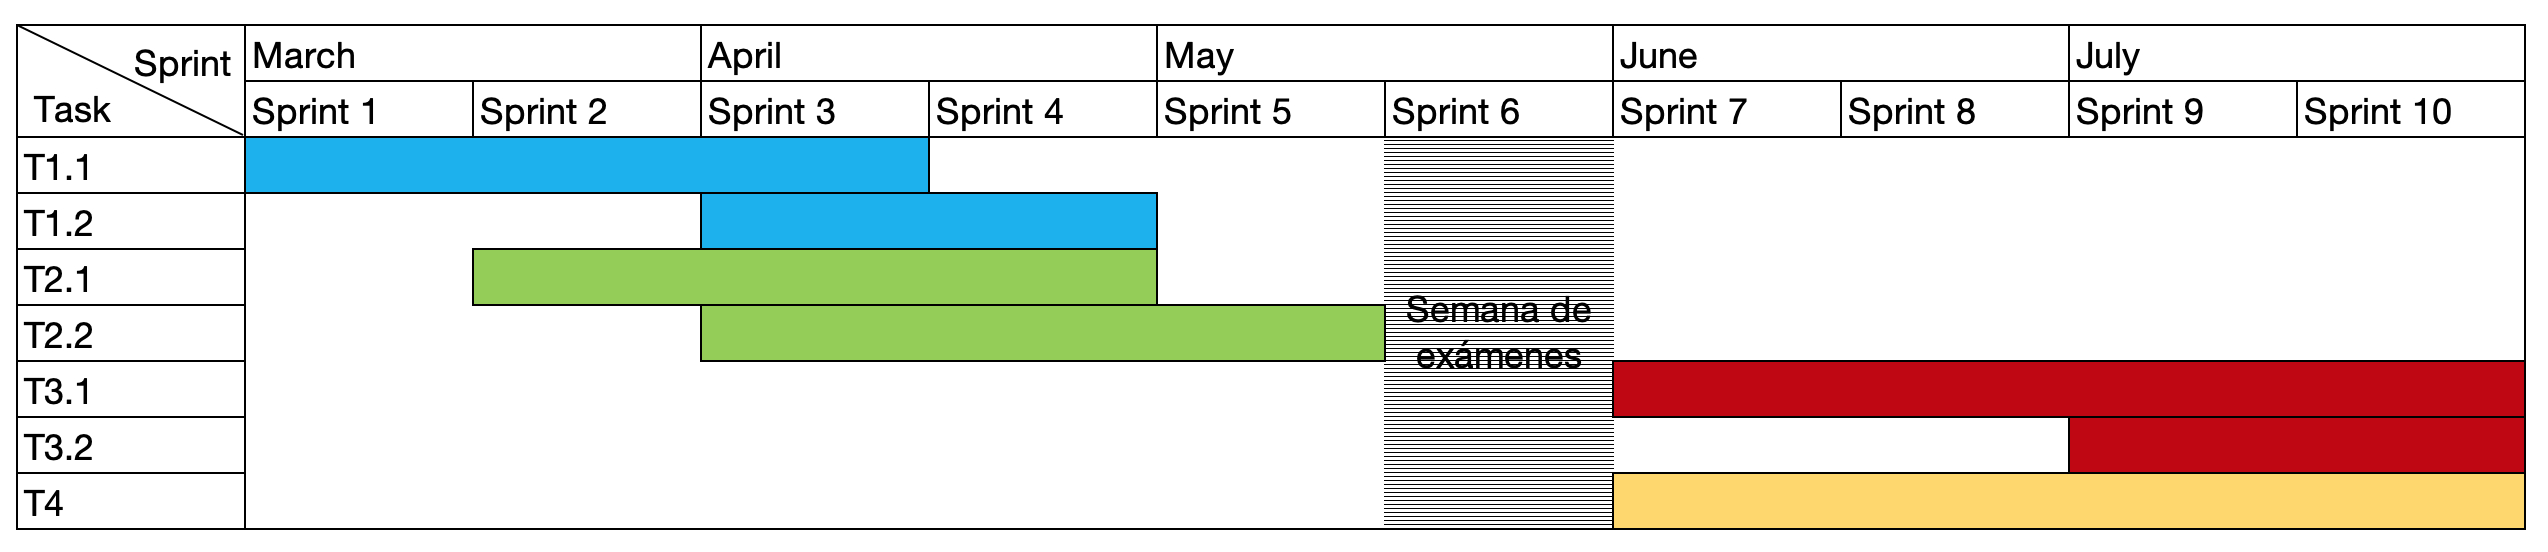
\includegraphics[scale=0.33]{images/planning/planning_gantt}}
\end{figure}
\chapter{Research methodology and implementation}



%----------
%	BIBLIOGRAFÍA
%----------	

%\nocite{*} % Si quieres que aparezcan en la bibliografía todos los documentos que la componen (también los que no estén citados en el texto) descomenta está lína

\clearpage
\addcontentsline{toc}{chapter}{Bibliography}
\printbibliography



%----------
%	ANEXOS
%----------	

% Si tu trabajo incluye anexos, puedes descomentar las siguientes líneas
%\chapter* {Annexes x}
%\pagenumbering{gobble} % Las páginas de los anexos no se numeran



\end{document}